\section{Proposal: Thermostat}
\label{proposal}

End-to-end Linux Prototype with minimal hardware changes to employ
slower but cheaper memory in data-centers.

\subsection{Identifying HotSpots in Cold Hugepages}

\begin{figure}[t]
\centering
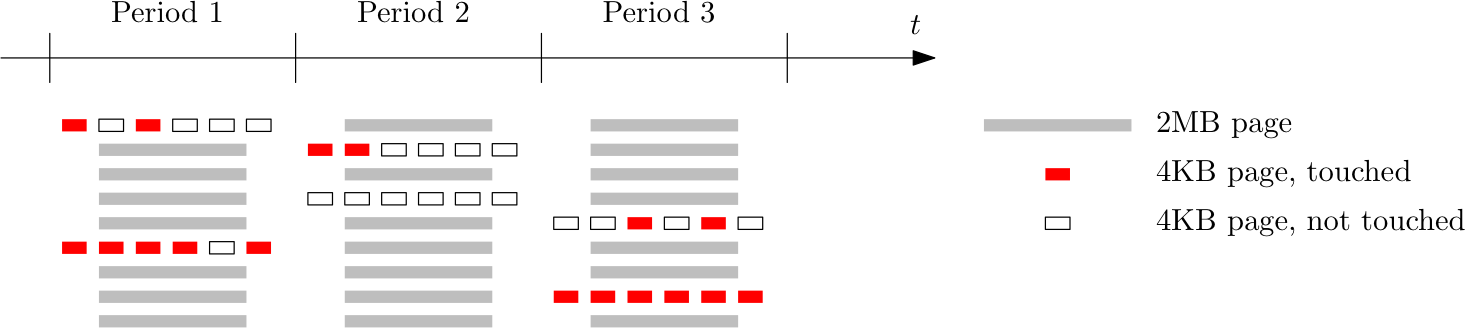
\includegraphics[width=1.0\columnwidth]{thermostat/figures/sampling.png}
\caption{Sampling to identify HotSpot pages in otherwise cold page}
\vspace{-0.175in}
\label{fig:sampling}
\end{figure}
To solve this situation, we propose to build a dynamic controller (which we call
Thermostat) that can decide when to {\it break} a huge page into several regular
pages, and place some of those smaller pages which are deemed to be cold in
slower but cheaper memory. We will implement Thermostat as a part of custom
Linux prototype. The following design issues arise when creating this Thermostat
controller.

First, the Thermostat controller has to distinguish between ``hotSpot'' hot pages -- ones
with only a few hot data blocks, and ``uniform'' hot pages -- ones where a
significant fraction of the data blocks in that page are hot.  We propose to
build such a classification mechanism that is at once a)
application-transparent, i.e., no source code change in the application should
be necessary, b) low-overhead, so as to not degrade the performance benefits of
using THP, and, c) high-accuracy, i.e., most of the classified ``hotSpot'' pages
are indeed hotspots (low false positives) and most of the pages classified
``uniform'' are {\it} not in fact hotspots (low false negatives).

We observe that there are hot 4KB pages present within 2MB huge pages.
Figure~\ref{fig:motivation-thermostat}
shows that applications on average have $\approx$ 50\% of cold data. As we change page size
form 4KB to 2MB fraction of cold data reduced by $\approx$ 50\%. Page granularity based
OS mechanisms cannot reveal the hot portions within huge pages. Hence, we
propose a sampling based page temperature measurement mechanism that classifies
pages by their access rate.

\subsection{Translation Facades}

%\begin{figure}[t]
%\centering
%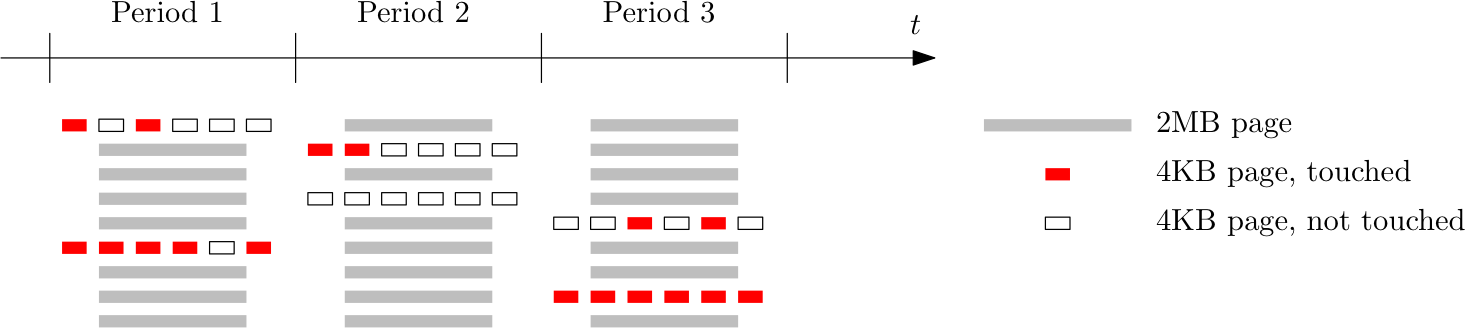
\includegraphics[width=1.0\columnwidth]{thermostat/figures/sampling.png}
%\caption{TLB and PTE changes}
%\vspace{-0.175in}
%\label{fig:motivation}
%\end{figure}
%
Second, the Thermostat controller needs an effective mechanism for chunking up a DRAM
huge page into several small pages, and also for compacting several small hot
pages into a single DRAM huge page. Chunking up a huge page is relatively simple
-- one need only allocate several page table entries (PTEs) corresponding to the
chunked up page. Doing the inverse, that is compacting several small pages from
the slow-mem and DRAM into a single DRAM huge page has more challenges. First,
due to memory fragmentation, it may not be possible to find a suitable space to
put the newly created huge page. Second, reading several small pages from
slow-mem, and creating a huge page out of them can be a potentially very long
latency operation, which can then affect application throughput as well as tail
latency. We plan to study the design trade-off space of when to perform
these operations and incorporate the obtained insights into building the Thermostat
controller.
